% Document class options:
% 11pt for 11 point font
% oneside for not weird margins between odd and even pages
% (omitting oneside gives a better margin setup for print
% but i'm guessing  you're handing this in)
% a4paper to A4 page size, because LaTeX by default is setup
% to use US Letter paper size, because Donald Knuth
% the article class, as the book class is designed for
% larger documents and you probably don't need chapter
% environments
\documentclass[11pt, oneside, a4paper]{article}
\usepackage[utf8]{inputenc}
\usepackage[english]{babel}
\usepackage[hypertexnames=false]{hyperref} 
\hypersetup{
    colorlinks=true,
    linkcolor=black,
    filecolor=magenta,      
    urlcolor=cyan,
}

\urlstyle{same}

\usepackage[utf8]{inputenc}
\usepackage{graphicx}
\usepackage{array}


% Set spacing (i set it to 1.2x)
\renewcommand{\baselinestretch}{1}
% Indentation (set this to zero for normal prose)
\setlength{\parindent}{0em}
% Line breaking (spacing between paragraphs)
\setlength{\parskip}{0.5em}

% Use the whole page
\usepackage{geometry}
% Extra math glyphs
\usepackage{amsmath}
% Proper enumerate spacing
\usepackage{enumitem}
% More pleasing screen fonts
\usepackage{lmodern}
% Fancy headers
\usepackage{fancyhdr}
\usepackage{graphicx}
% Allows absolute positioning of images
\usepackage{float}
% \usepackage[section]{placeins}
% Set no separation
\setlist{noitemsep}
% Set margins to reasonable
\geometry{margin=2.5cm}
% Sets graphics path
\graphicspath{ {./images/} }
% Sets up fancy headers

\addto\captionsenglish{
\renewcommand{\listfigurename}{List of Images}
}


\usepackage{listings}
\usepackage{color}

\pagestyle{plain}

\begin{document}


\definecolor{dkgreen}{rgb}{0,0.6,0}
\definecolor{gray}{rgb}{0.5,0.5,0.5}
\definecolor{mauve}{rgb}{0.58,0,0.82}

\lstset{frame=tb,
  language=Python,
  aboveskip=3mm,
  belowskip=3mm,
  showstringspaces=false,
  columns=flexible,
  basicstyle={\small\ttfamily},
  numbers=none,
  numberstyle=\tiny\color{gray},
  keywordstyle=\color{blue},
  commentstyle=\color{dkgreen},
  stringstyle=\color{mauve},
  breaklines=true,
  breakatwhitespace=true,
  tabsize=3
}

\pagestyle{fancy}
\fancyhf{}
\lhead{Natalie Hong - Visualisation Report}
\rhead{COSC3000}

\begin{titlepage}
\newgeometry{left=7.5cm} %defines the geometry for the titlepage
\noindent
\color{black}
\makebox[0pt][l]{\rule{1.3\textwidth}{1pt}}

{\Huge {Natalie Hong (45309740)}}
\vskip\baselineskip
\noindent
{\huge{COSC300 Graphics Report}}

\vskip\baselineskip
{\large {Semester 1 - 2020}}
\end{titlepage}

\newpage
\tableofcontents

\listoffigures

\newpage


\section{Introduction}
In this document, you will find my findings and attempts at creating a completed game. The game I had chosen to make was that of the supplied mega racer code.

\subsection{Problem Statement}
The problem I had was that of not knowing enough computer graphics knowledge to create a full game. Through the development of the mega racer game, I aimed to improve my understanding of computer graphics as well as create a fun, nice-looking and interactive game for users to play.

\subsection{Methods, Techniques and Execution}
To create the graphics required for this project, I used Python 3.5 and OpenGL to create objects and renderables within the computer graphics scene. I also used GitHub to allow for version control between each implemented feature that I added.

The features that were made were:
\begin{itemize}
	\item{2 - Scaling the Terrain}
	\item{3 - Setting up the Camera}
	\item{4 - Orientating and Placing the Racer Model}
	\item{5 - Texturing the Terrain}
	\item{6 - Lighting from the Sun}
	\item{7 - Improving Textures}
    \item{8 - Adding Fog}

\end{itemize}


In the following documentation, you will find screenshots and findings which include results and discussion around each feature as well as how I went about approaching each feature within the project. 

\section{Scaling the Terrain}
Scaling terrain consisted of scaling the terrain according to the path image supplied.
\begin{lstlisting}    
	# copy pixel 4 channels
        imagePixel = self.imageData[offset:offset+4];
        # Normalize the red channel from [0,255] to [0.0, 1.0]
        red = float(imagePixel[0]) / 255.0;

        xyPos = vec2(i, j) * self.xyScale + xyOffset;
	# TODO 1.1: set the height
	zPos = 0
\end{lstlisting}

Initially, the code supplied consisted of zPos = 0 and I was to change it. I thought long and hard about to change and looked at the hints supplied. In it, I was told to use self.heightScale and to somehow utilize it in order to get a consistent z position for each terrain created. I had a thought that multiplying the red value calculated would allow me to get a a consistent z position. This was because red represented a value from 0 to 255 and multiplying it with the height scale would allow for different Z positions to be generated.

\newpage
\begin{lstlisting}    
	# TODO 1.1: set the height
	zPos = self.heightScale * red
\end{lstlisting}

\begin{figure}[!ht]
	\centerline{
\includegraphics[scale=0.35]{/2_1.png}}
	\caption{Scaled Terrain}
	\label{fig:figure1}
\end{figure}

This seemed to work as I was now able to see bumps and curves within the terrain which meant this feature was completed.

\section{Setting up the Camera}
The next feature I was to implement was that of setting up the camera so that it viewed the racer at all times and was scaled to the supplied camera offset. As well as this, I wanted the camera to be able to rotate according to the heading of the racer. After much experimentation I was able to come up with the following code:

\begin{lstlisting}  
    x = g_racer.position[0]
    y = g_racer.position[1]
    z = g_racer.position[2]

    ....
    g_viewTarget = [x, y, z]
\end{lstlisting}

\begin{figure}[!ht]
	\centerline{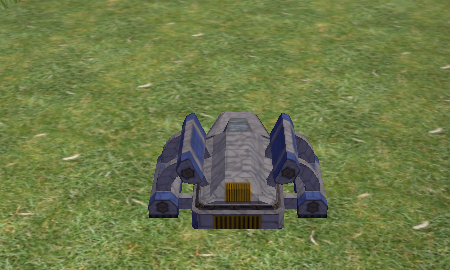
\includegraphics[scale=0.35]{/3_1.png}}
	\caption{Looking at the Racer}
	\label{fig:figure2}
\end{figure}

Since I wanted my camera to look at the racer, I decided to make it so that the camera was always looking at where the racer was positioned. However, I did not want the camera to be at the exact same position as the racer as that would make it feel weird. To make sure the camera was positioned away from the racer, I used the assigned follow cam offsets. This code was very similar to Lab 3 of the course. The result can be seen in the above figure, please note that this screenshot was taken later into development of the game.

\begin{lstlisting}  
    for i, positionPoint in enumerate(g_racer.position): 
        g_viewPosition[i] = positionPoint + g_followCamOffset * -g_racer.heading[i]

    g_viewPosition[2] += g_followCamLookOffset
\end{lstlisting}
In the code above, I was able to create a viewing position for the camera to be positioned at. Position points were each of the racer's coordinates and were then added to the follow cam offset multiplied by the negative of the racer's heading coordinates. Since -1 for the heading coordinates corresponded to the right rather than the left, I made sure to make the values reverse using the negative version of the heading value.

Since z-axis had an added follow camera offset as it was specified in the task sheet, I made sure that the z axis needed to have the additional multiplier of the follow cam offset to it.

\begin{figure}[!ht]
	\centerline{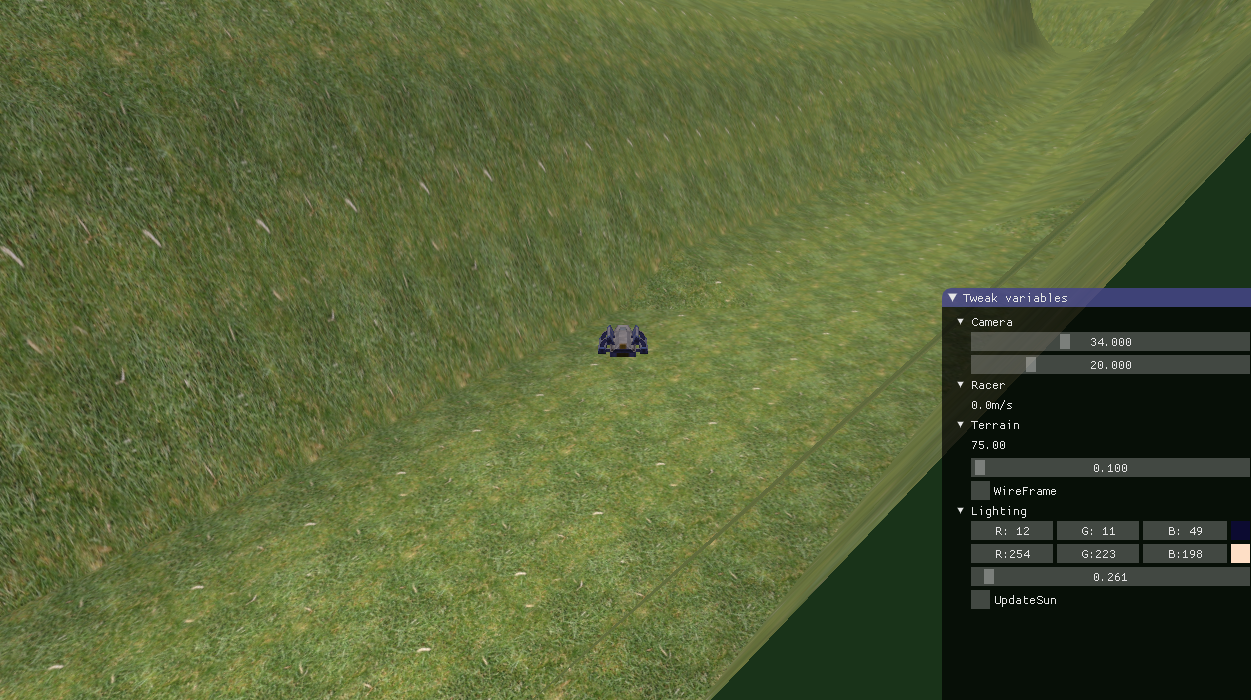
\includegraphics[scale=0.35]{/3_2.png}}
	\caption{Camera Rotating with the Racer}
	\label{fig:figure3}
\end{figure}
The result of rotating the camera can be seen in the above figure, please note that this screenshot was taken later into development of the game.

\section{Orientating and Placing the Racer Model}
This task for the racer required me to rotate and orientate the model. This model loading was very similar to the of Lab 1. To place the model at the racer's location I did the following:

\begin{lstlisting}  
        top = [0,0,1] # Define top in the Z-axis
        modelInWorld = lu.make_mat4_from_zAxis(self.position, self.heading, top)
        # Draw model in the specified world coordinates
        renderingSystem.drawObjModel(self.model, modelInWorld, view) 
\end{lstlisting}

First, I defined the top of the world in that of the z-axis. This was necessary as the task sheet recommended to do it and allowed me to use more functions. Using this top value, I made a 4x4 matrix using the racer's position, where it was heading and the top value defined earlier. Once I got this 4x4 matrix which represented coordinates to draw the model in, I then added the model to the coordinates and used the passed in view to place the Racer in the scene. 

\begin{lstlisting}  
	self.model = ObjModel(objModelName)
\end{lstlisting}

The last thing I did was load the model inside the racer's load function so the racer model could initialise on load. 

\begin{figure}[!ht]
	\centerline{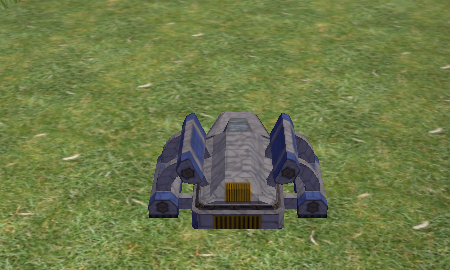
\includegraphics[scale=0.35]{/4_1.png}}
	\caption{The Loaded Model}
	\label{fig:figure4}
\end{figure}
Once loaded, I was able to rotate the model with the camera to allow for the racer model to always be facing forwards no matter which way the camera was adjusted to.

\section{Texturing the Terrain}
As you may have seen in previous figures, I was able to texture the terrain of the game. This was done by binding textures to a variable to create unique texturing for the grass and to allow for more 

\begin{lstlisting}  
   # Texture ids
    grassId = None

    # Texture unit allocations:
    TU_Grass = 0
\end{lstlisting}

First, I defined a grassId to use and bind a texture to. I also loaded the texture from the path (grass2.png) after I defined the texture. This was so that I could get the actual image to show.
 
\begin{lstlisting}  
        #TODO 1.4: Bind the grass texture to the right texture unit, hint: lu.bindTexture
        lu.bindTexture(self.TU_Grass, self.grassId)
        lu.setUniform(self.shader, "grassId", self.TU_Grass)
        ...
        self.grassId = ObjModel.loadTexture("data/grass2.png", basePath, True)
\end{lstlisting}

I then used similar code to that of the fifth and fourth lab (the ones about textures and lighting), to create a texture definition for the grass.

To do this, I translated the texture using the binded grass id to a texture and passed in the world space position and multiplied it with the xy texture scale. I did this to make sure that the terrain would be scaled to my game's world. I then was able to get a grass colour using this texture function which I then passed into compute the shading that the grass would be according to the light given from the sun.

I then was able to finally convert the reflected light into a fragment color variable which would serve as the level of light that the grassId texture was to give off.

\begin{lstlisting}  
        void main() 
         {
             vec2 testvecw = v2f_worldSpacePosition.xy;
            
             vec3 materialColour = vec3(v2f_height/terrainHeightScale);
                
             // TODO 1.4: Compute the texture coordinates and sample the texture for the grass and use as material colour.
             vec3 grassColour = texture(grassId, testvecw * terrainTextureXyScale).xyz;
             vec3 reflectedLight = computeShading(grassColour, v2f_viewSpacePosition, v2f_viewSpaceNormal, viewSpaceLightPosition, sunLightColour);
	      fragmentColor = vec4(toSrgb(reflectedLight), 1.0);

         }
\end{lstlisting}
 
 The end result looked like the following:
 \begin{figure}[!ht]
	\centerline{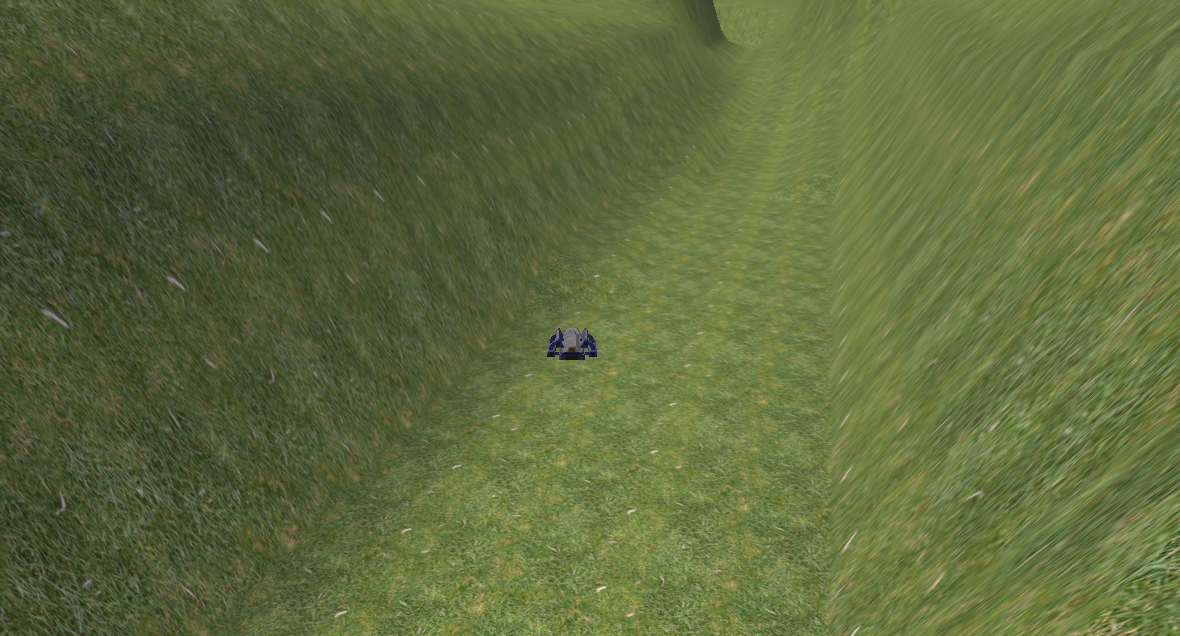
\includegraphics[scale=0.35]{/5_1.png}}
	\caption{The Textured Terrain}
	\label{fig:figure5}
\end{figure}

\section{Lighting from the Sun}
Using the shaders supplied from lab 4, I was able to create similar shaders for the sun. For part where I was supposed to add code, I noticed that the passed in variables were:
\begin{itemize}
	\item{vec3 materialColour}
	\item{vec3 viewSpacePosition}
	\item{vec3 viewSpaceNormal}
	\item{vec3 viewSpaceLightPos}
	\item{vec3 lightColour}
	\item{global variable of globalAmbientLight}
\end{itemize}

These variables were very similar to the shaders in lab 4 so I used them as reference. Since there was no material alpha for the object like the previous labs, I decided to not add any extra variables to create this. The explanation for each step I took can be seen in the code block below.

\begin{lstlisting}  
vec3 computeShading(vec3 materialColour, vec3 viewSpacePosition, vec3 viewSpaceNormal, vec3 viewSpaceLightPos, vec3 lightColour)
    {
        # TODO 1.5: Here's where code to compute shading would be placed most conveniently
        # Compute incoming light, stop complete blackness when the sun is hidden
        vec3 viewSpaceDirToLight = 	normalize(viewSpaceLightPos - viewSpacePosition);
        float incomingIntensity = max(0.0, dot(viewSpaceNormal, viewSpaceDirToLight));
        # Get the yellow-ish tinge from the sun's incoming light
        vec3 incomingLight = incomingIntensity * lightColour;
        # Add directional light
        vec3 outgoingLight = (incomingLight + globalAmbientLight) * materialColour;
        return outgoingLight;
    }
\end{lstlisting}

This meant that the sun was able to update according to the sunAngle which was later used to calculate the values viewSpaceLightPosition, sunLightColour and globalAmbientLight which were passed into the shader code during the sun's update function. My game was able to look like the following:

\begin{figure}[H]
    \centering
    \begin{minipage}{0.5\textwidth}
        \centering
        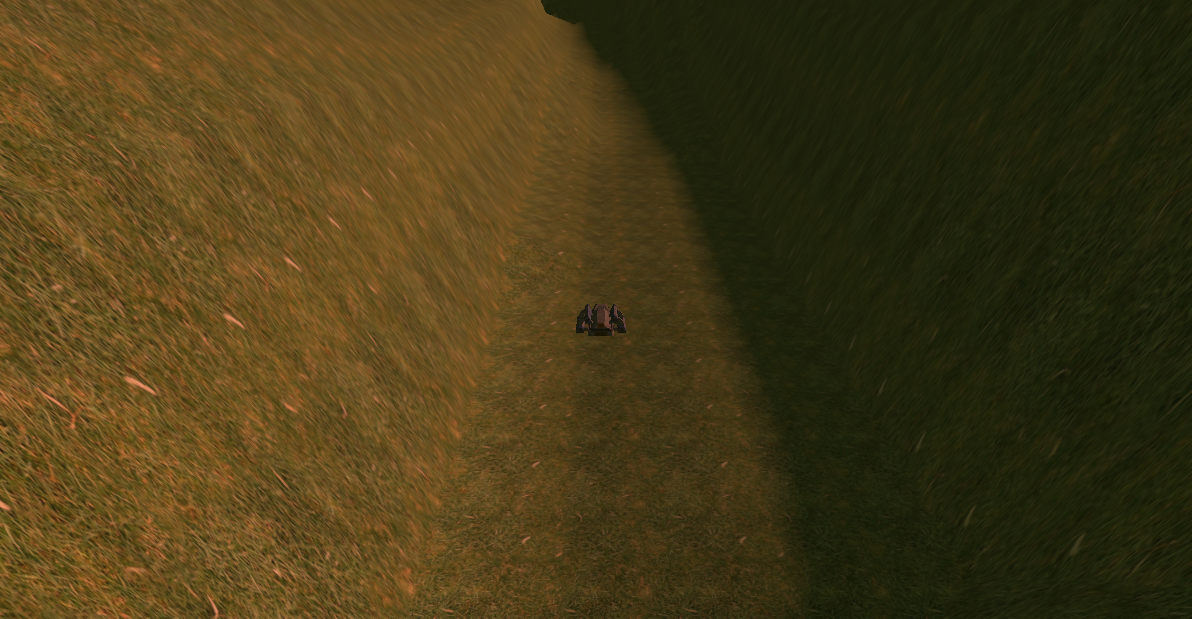
\includegraphics[width=0.9\linewidth]{/6_2.png}
        \caption{Afternoon Sun Look}
    \end{minipage}%
    \begin{minipage}{0.5\textwidth}
        \centering
        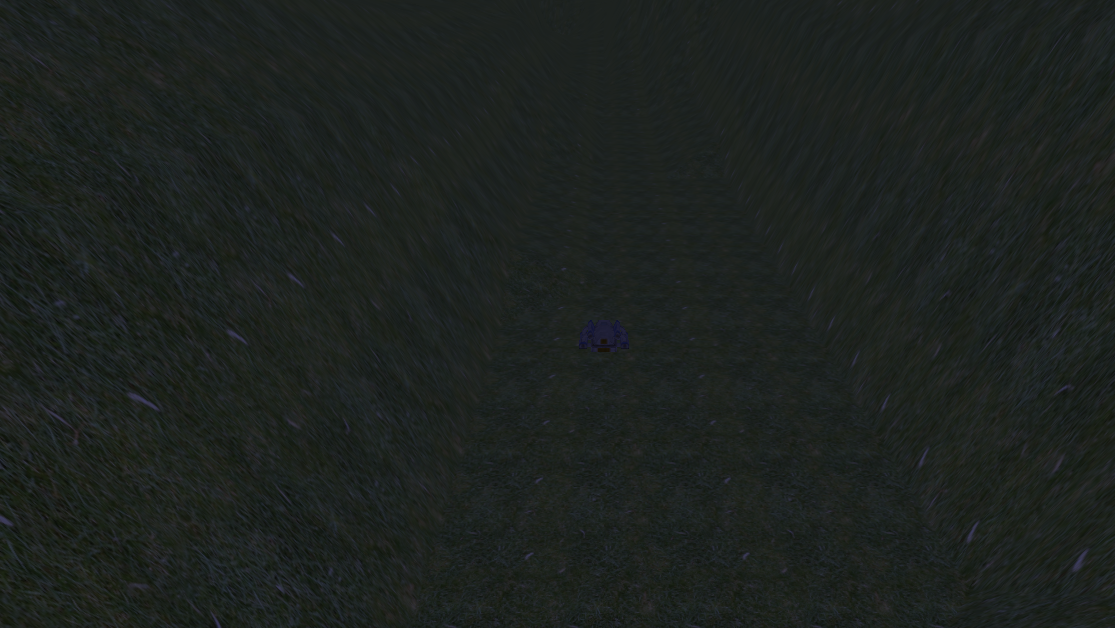
\includegraphics[width=0.9\linewidth]{/6_1.png}
        \caption{No Sun}
    \end{minipage}
\end{figure}

\newpage
\section{Improving Terrain}
Improving terrain according to the task sheet was that of adding different terrain textures to the game which coicided with that of higher rocks, steeper rocks and a road. 

To start off, I defined some texture ids and texture variables to bind the new textures to alongside the existing grass texture one. I also loaded the texture from the path similar to that of the was I loaded the grass path.
\begin{lstlisting}
# Texture ids
grassId = None
highRockId = None
steepRockId = None
roadId = None

# Texture unit allocaitons:
TU_Grass = 0
TU_High_Rock = 1
TU_Steep_Rock = 2
TU_Road = 3

...
#TODO 2.1: Improve Terrain Textures
self.highRockId = ObjModel.loadTexture("data/rock 2.png", basePath, True)
self.steepRockId = ObjModel.loadTexture("data/rock 5.png", basePath, True)
self.roadId = ObjModel.loadTexture("data/paving 5.png", basePath, True)
\end{lstlisting}

I went by the task sheet's hint of using the height variable in the shader to define the material colour at when the height was above 60 to be that of the high rock texture.

\begin{lstlisting}
if (v2f_height > 60) {
    materialColour = texture(highRockId, testvecw * terrainTextureXyScale).xyz;
} 
\end{lstlisting}

Calculating the steep rocks proved to be a bit of a challenge as I was not too sure on where to start. I searched up on the internet on how to find the angle between two vectors (that of the  z-axis/flat ground and the worldSpaceNormal as specified in the spec). I was fortunate to come across a \href{https://stackoverflow.com/questions/41984724/calculating-angle-between-two-vectors-in-glsl}{Stack Overflow} question which was very related to what I wanted to do. I then found the normal of the z-axis and that of the world space and applied the dot product to the vectors. I then found the acos of the dot product to find the angle. The code looked like the following and was then used to determine steep slopes within the terrain:

\begin{lstlisting}
    vec3 worldSpace_Normal = normalize(v2f_worldSpaceNormal); // Normal of world space
    vec3 zaxis_Normal = normalize(vec3(0, 0, 1)); // Normal of Z-axis
    float angle = acos(dot(worldSpace_Normal, zaxis_Normal));
    ...
    if (angle > 0.45) { // Angled
        materialColour = texture(steepRockId, testvecw * terrainTextureXyScale).xyz;
    }
\end{lstlisting}

\newpage
\begin{figure}[!ht]
	\centerline{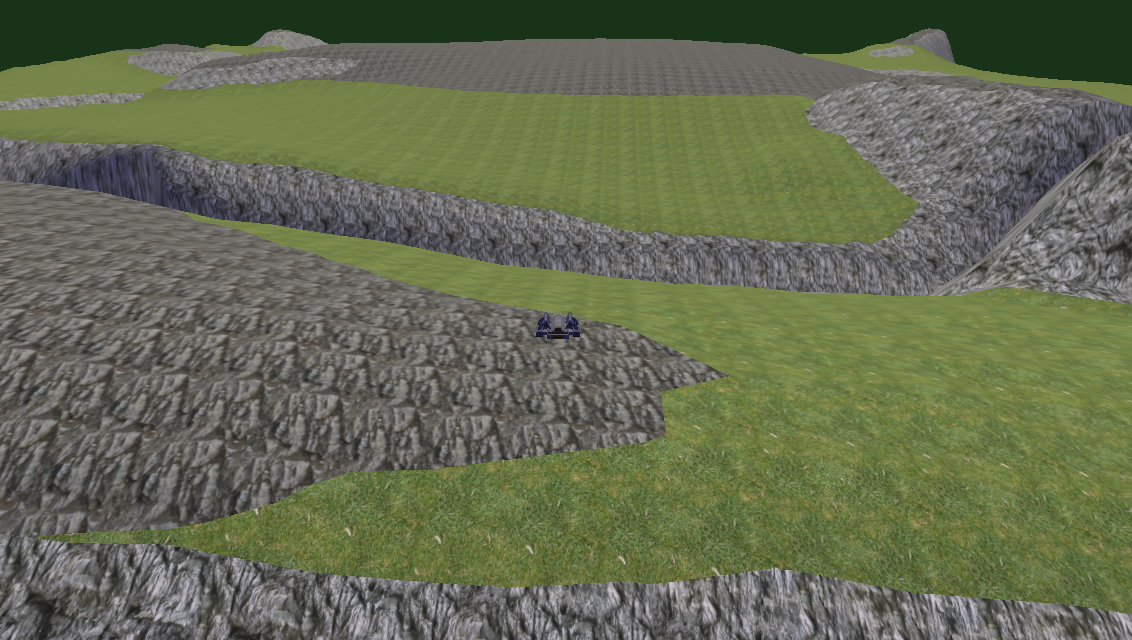
\includegraphics[scale=0.35]{/7_2.png}}
	\caption{The Textured Terrain}
	\label{fig:figure5}
\end{figure}

With the high stones and the steep stones done, I was then to do the road. From what the task sheet said, I was to use the rgb pixels to determine where the road was to be placed. This turned out to be a little harder to do and I was unsure on how to correctly implement this, so I decided to approach it in my own way.

Similar to the way I did the steep stones, I checked with the height threshold but instead I used height less than rather than greater than. 

\begin{lstlisting}
    if (v2f_height < 30) {
        materialColour = texture(roadId, testvecw * terrainTextureXyScale).xyz;
    } 
\end{lstlisting}

\begin{figure}[!ht]
	\centerline{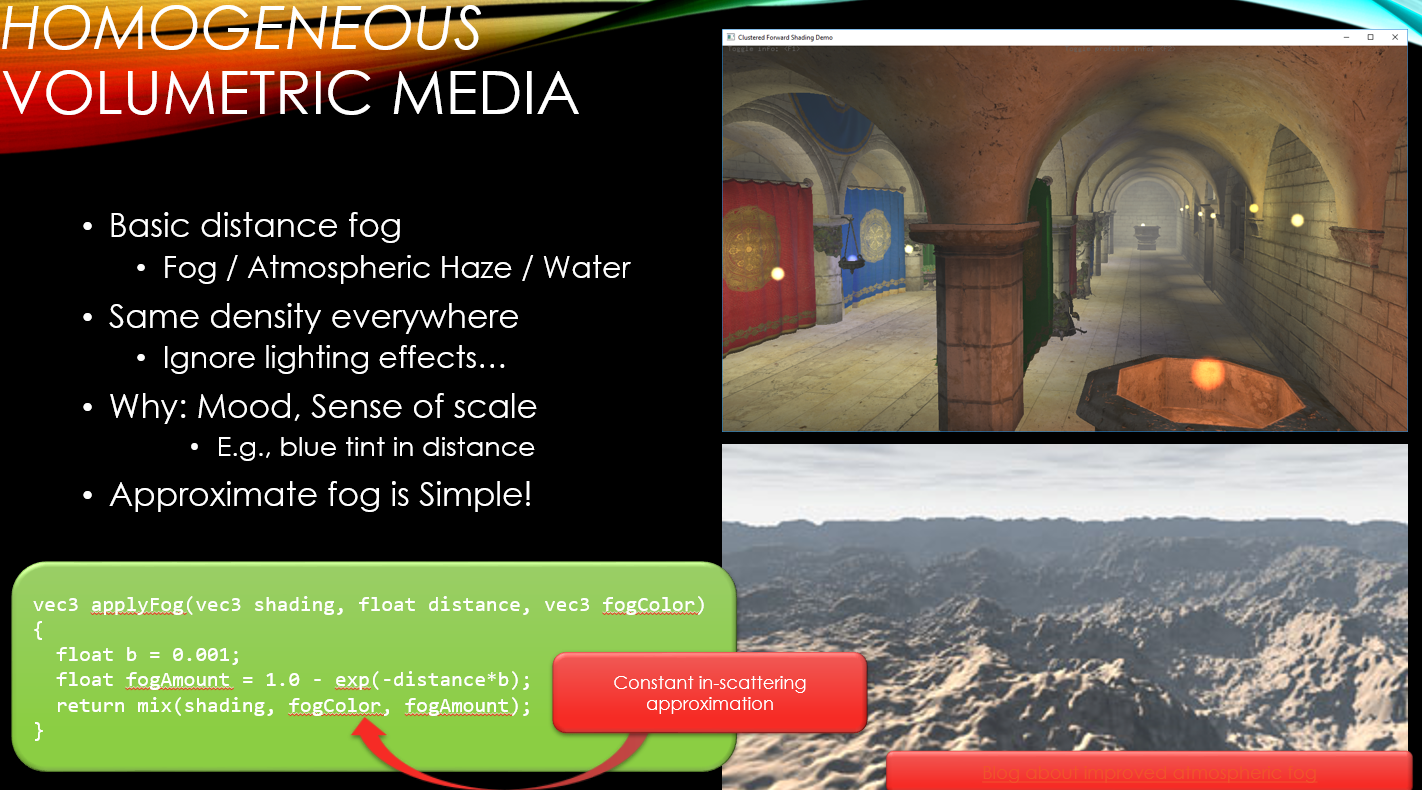
\includegraphics[scale=0.35]{/7_1.png}}
	\caption{The Textured Terrain}
	\label{fig:figure5}
\end{figure}
This allowed me to get a semi-functional road, although it did vary in length at some points which was due to the height factor not being enough to calculate it. I felt like this approach was suitable though was the road was still visible within the track and looked nice.

\newpage
\section{Adding Fog}
When I was watching lectures for this course, I noticed that one of the lecture slides had a link to a helpful website that I could use. 

\begin{figure}[!ht]
	\centerline{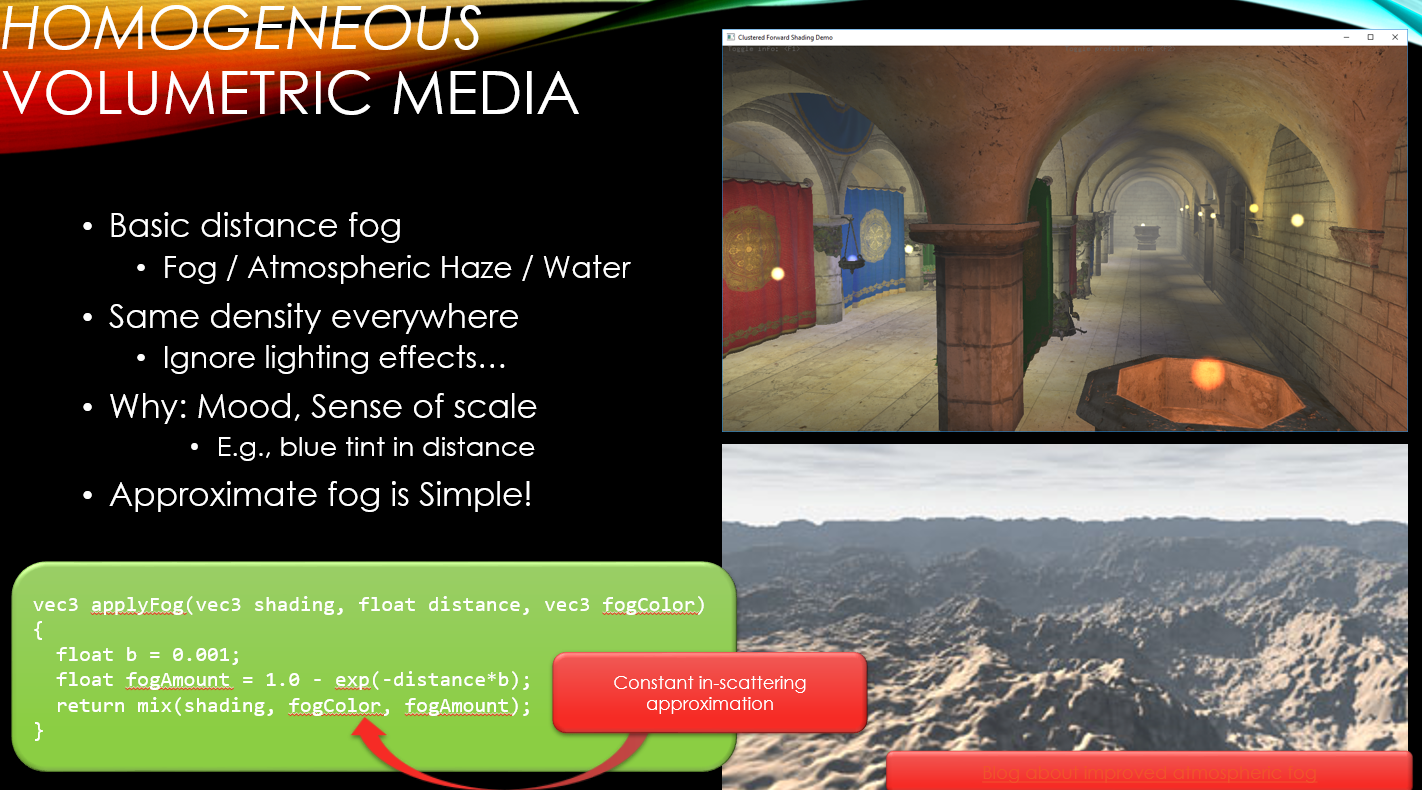
\includegraphics[scale=0.35]{/8_1.png}}
	\label{fig:figure10}
\end{figure}

When I went to the \href{https://iquilezles.org/www/articles/fog/fog.htm}{website}, I was able to find some interesting information on how to implement fog. 

\begin{figure}[H]
    \centering
    \begin{minipage}{1\textwidth}
        \centering
        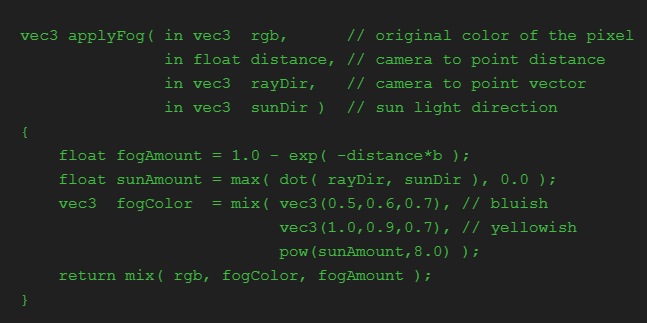
\includegraphics[width=0.75\linewidth]{/8_2.png}
        \caption{First Look}
    \end{minipage}
    \begin{minipage}{1\textwidth}
        \centering
        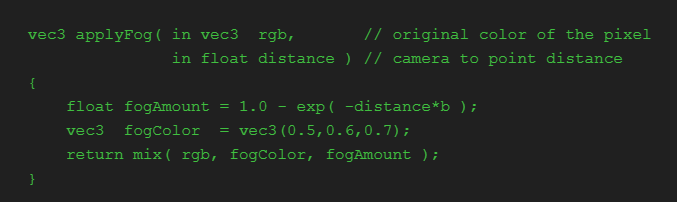
\includegraphics[width=0.75\linewidth]{/8_3.png}
        \caption{Final Decision}
    \end{minipage}
\end{figure} 

As seen in Figure 8, the code demonstrated was that of an apply fog function that was to be put in the megaracer file. I initially tried to implement this function but was unsure about the rayDir and sunDir variables that were passed into it. I originally tried passing in viewSpacePosition and viewSpaceLightPosition which did not seem to do what I wanted as the sun did not end up shaded properly for some reason.

So instead I with the approach seen in Figure 9. Once I had impmented this, I realised that the fog was kept to one colour as the fogColor variable was kept constant and turned out to just be grey which did not give too much volume to it. 

I tried adding sunLightColour to be the new fog colour but that seemed to make the fog colour only be independently influenced by the sun, which I did not want. So I decided to combine it with the global ambient light colour as per the specification task.

\begin{lstlisting}
    vec3 applyFog(in vec3 rgb, in float distance) {
        float b = 0.0045; 
        float fogAmt = 1.0 - exp(-distance*b);
        vec3  fogColor = (sunLightColour + globalAmbientLight);
        return mix(rgb, fogColor, fogAmt);
    }
\end{lstlisting}

My apply fog function now looked like this. Using the code that was from the lecture slides (Figure 8), I was able to add fog to my game's code which looked like the following:

\begin{lstlisting}
    // Applying fog
    // reflectedLight - rgb pixel colour
    // v2f_viewSpacePosition.z - Distance
    fragmentColor = vec4(toSrgb(applyFog(reflectedLight,
            v2f_viewSpacePosition.z)), 1.0);
\end{lstlisting}

This however, resulted in my game looking like the following:
\begin{figure}[!ht]
	\centerline{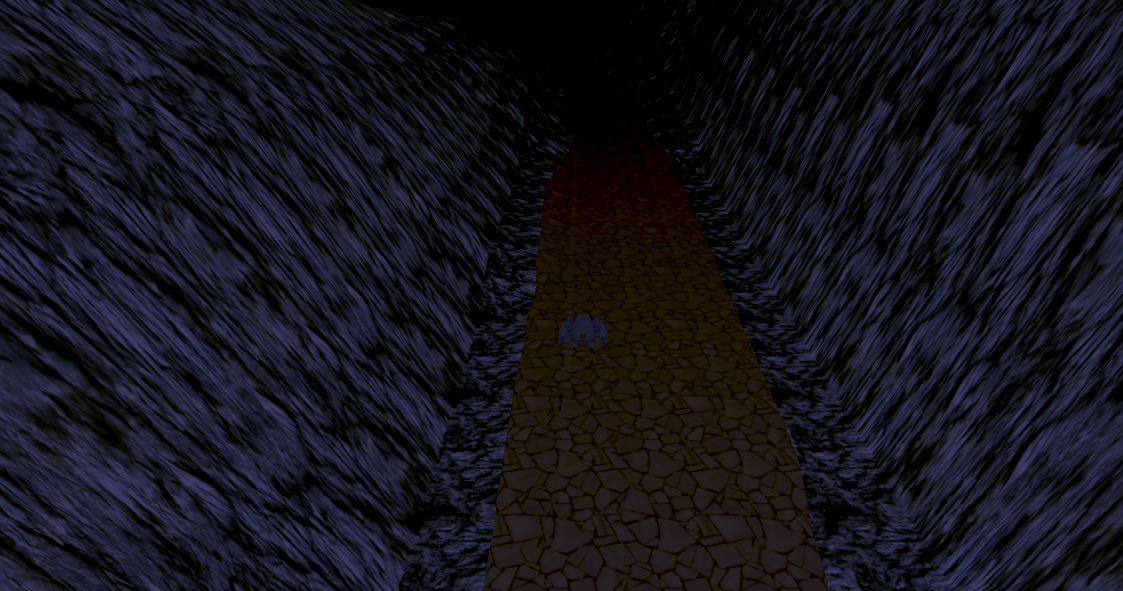
\includegraphics[scale=0.35]{/8_4.png}}
	\caption{The Incorrectly Shaded Fog}
	\label{fig:figure10}
\end{figure}

\newpage
I figured that this was happening as the distance in the applyFog function was making a negative version of the distance that was passed into it. To fix this, I simply had to change from this:
\begin{lstlisting}
    float fogAmt = 1.0 - exp(-distance*b);
\end{lstlisting}
To this:
\begin{lstlisting}
    float fogAmt = 1.0 - exp(distance*b);
\end{lstlisting}

\begin{figure}[!ht]
	\centerline{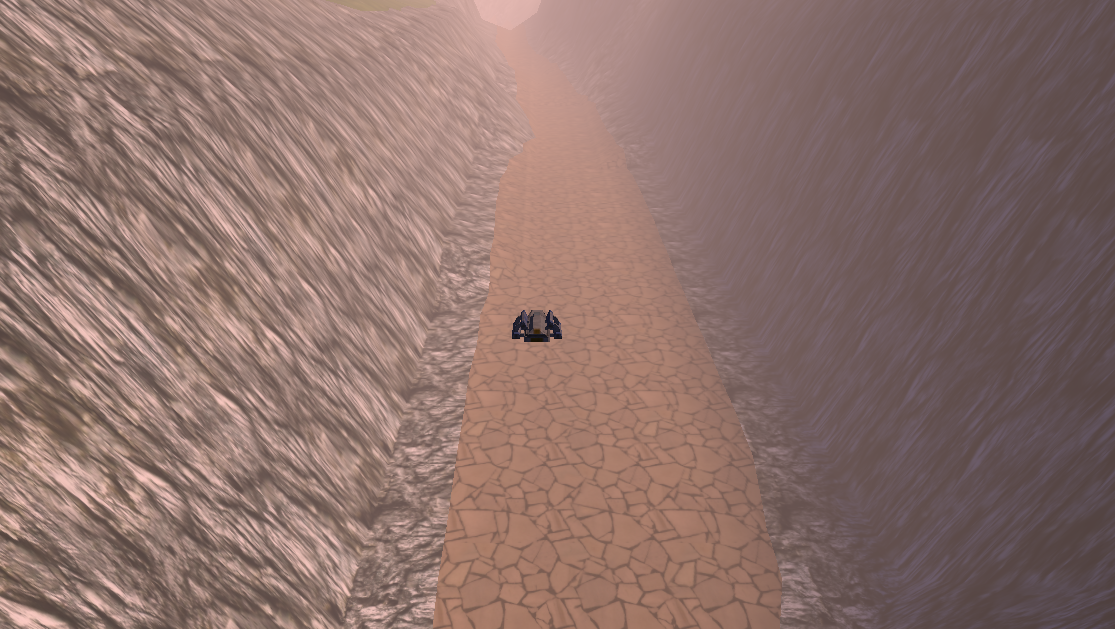
\includegraphics[scale=0.35]{/8_5.png}}
	\caption{The Correctly Shaded Fog}
	\label{fig:figure10}
\end{figure}
The correctly shaded fog looked like that seen in Figure 11, this fog stayed constant throughout the sun cycle in the game and allowed for depth in the game to be seen more clearly.



\end{document}

















